\documentclass[12pt, letterpaper]{article}
\usepackage[spanish]{babel}
\usepackage[utf8]{inputenc}
\usepackage{graphicx}
\usepackage{amssymb}
\graphicspath{{./imagenes/}}

%Paquetes para símbolos y entornos matematicos. En este documento se usa para poder usar el tag \begin{align} y \begin{align*} que permiten alinear expresiones matemáticas
\usepackage{amsmath}
\usepackage{amssymb}
%paquete que permite el uso de del argumento H al momento de insertar imágenes
\usepackage{float}

%comando para especificar el título del documento 
\title{Matemáticas para las Ciencias Aplicadas I}

%comando para especificar el autor del documento
\author{Pérez Romero Natalia Abigail}

%comando para especificar la fecha del documento
\date{\today}
%--------------Fin preámbulo--------------

%------------Inicio documento-------------
\begin{document}
%comando que genera el titulo con los datos especificados en el preámbulo
\maketitle
\textbf{Tarea IV. Ejercicios del libro Cálculo. Una variable de Thomas J.R, George B.}

Ejercicios 1.3

\textbf{Funciones}
Encuentre el dominio y grafique cada función, agregando la precisión de máximo dominio donde la función esté bien definida.

(1) $f(x) = 1 + x^2$

El dominio de la función es $(-\infty , \infty)$ es decir  $\mathbb{R}$, dado que la funcion no tiene restricción.
\begin{figure}[h]
\centering
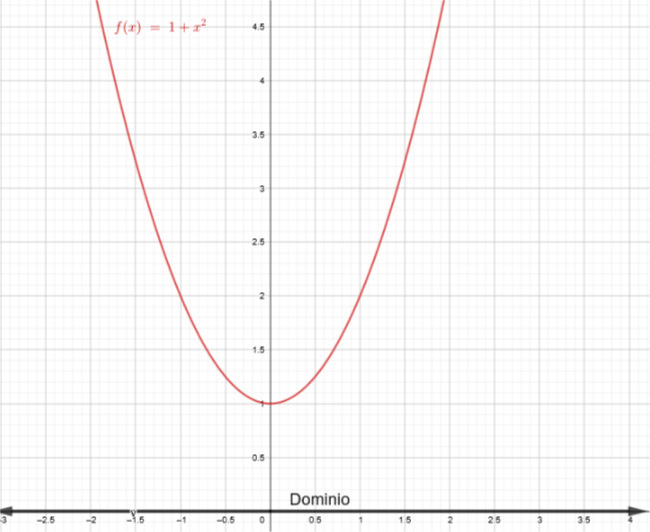
\includegraphics[width=20em]{uno}
\end{figure} 

\newpage
(2) $f(x) = 1 - \sqrt{x}$

Para que la imagen de $f(x)$ se mantenga en los reales $x$ debe ser mayor o igual a 0. Por lo tanto el dominio de $f(x)$ es $[0, \infty), \{x|x\geq 0\}$
\begin{figure}[h]
\centering
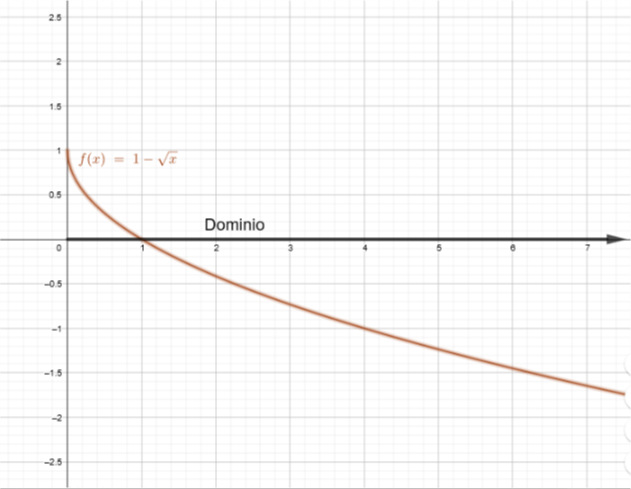
\includegraphics[width=20em]{dos}
\end{figure} 

(4) $F(t) = \frac{1}{1 + \sqrt{t}}$

Para que la imagen de $F(t)$ se mantenga en los reales $t$ debe ser mayor o igual que $0$. Por lo tanto el dominio de $F(t)$ es $[0, \infty), \{x|x\geq 0\}$
\begin{figure}[h]
\centering
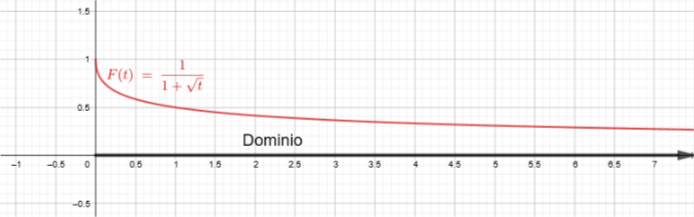
\includegraphics[width=20em]{tres}
\end{figure} 

\newpage

(17) $g(x) = \sqrt{|x|}$

Para que la imagen de $g(x)$ se mantenga en los reales x debe ser mayor o igual que $0$. Tomando en cuenta que $|x| = a \iff x = \pm a $. El dominio de $g(x)$ es $(-\infty, \infty)$, es decir, $\mathbb{R}$

\begin{figure}[h]
\centering
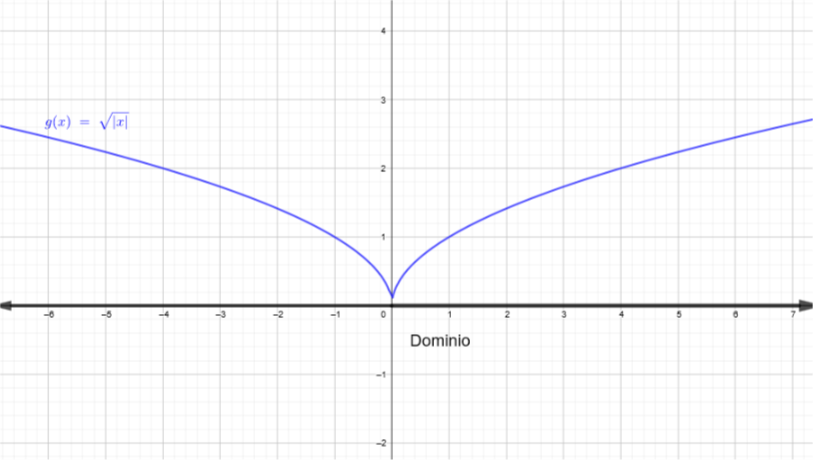
\includegraphics[width=20em]{cuatro}
\end{figure} 

(19) $F(t) = \frac{t}{|t|}$

Para que la imagen de $F(t)$ se mantenga en los reales x debe ser diferente a $0$. Tomando en cuenta que $|x| = a \iff x = \pm a $. El dominio de $F(t)$ es $(-\infty, 0)\cup(0,\infty)$, $\{x|x\neq0\}$

\begin{figure}[h]
\centering
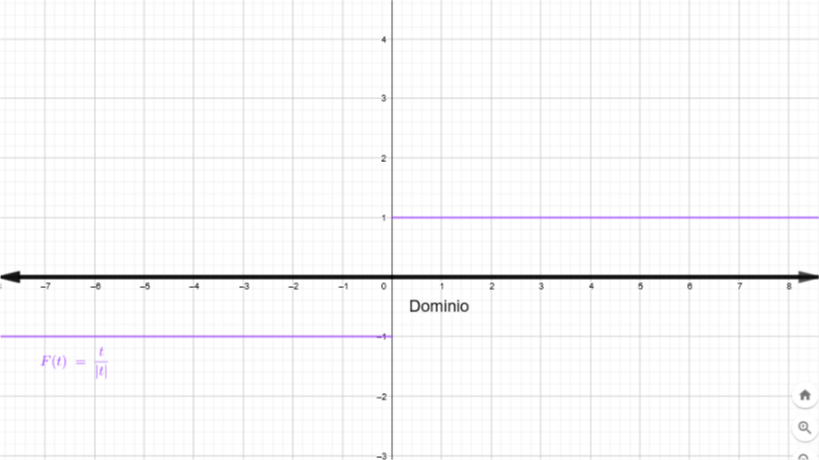
\includegraphics[width=20em]{cinco}
\end{figure} 

\newpage

De las gráficas siguientes determine cuáles corresponden a funciones de  $x$, así como cuáles de ellas no.
Una función $f$ sólo puede tener un valor $f(x)$ para cada $x$ en su dominio, de manera que ninguna \textit{recta vertical} puede intersecar más de una vez la gráfica de una función.

Trace varias rectas verticales en las siguientes gráficas, con lo que pude observar  que solo la gráfica 7.b es la gráfica de una función.
\begin{figure}[h]
\centering
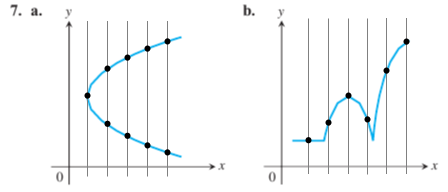
\includegraphics[width=30em]{siete}
\end{figure} 

\begin{figure}[h]
\centering
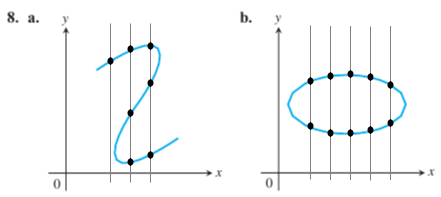
\includegraphics[width=30em]{ocho}
\end{figure} 

\newpage

Encuentre una fórmula para cada función graficada.
\begin{figure}[h]
\centering
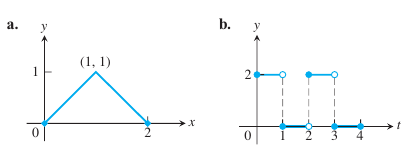
\includegraphics[width=30em]{veinticiete}
\end{figure} 

(a)
$$f(x) = \left\{
\begin{array}{c l}
 x & 0 \leq x \leqq 1\\
 2-x & 1< x \leqq 2
\end{array}
\right.
$$

(b)
$$g(x) = \left\{
\begin{array}{c l}
 2 & 0 \leq x < 1\\
 0 & 1 \leq x < 2\\
 2 & 2 < x < 3\\
 0 & 3 \leq x \leqq 4
\end{array}
\right.
$$

\end{document}
%----------Fin del documento--------------